
	\begin{enumerate}
		\item Цель:
		\begin{itemize}
			\item Реализовать ножничный подъемник, механизм, приводящий его в движение и закрепление на конструкции робота
			\item Написать программу для управления захватом с отдельного геймпада
		\end{itemize}
		\item Результаты:
		\begin{itemize}
			\item Робот был частично разобран из-за недостатка деталей, была собрана примерная схема механизма передвижения подъемника(Рисунок 6)
			\item Написать и отладить программу не получилось, опять же из-за отсутствия деталей
			\item При тестировании барабана для намотки лески обнаружился очень сильный изгиб конструкции во время вращения барабана. Возможно, проблема в неоткалиброванном барабане или осях моторов, находящихся на разных уровнях. Попытаемся исправить это на следующем занятии.
		\end{itemize}
		\item Идеи:
		\begin{itemize}
			\item Заменить текущие рейки в подъемнике на алюминиевые профили для удобства установки, увеличения длины составляющих подъемника и уменьшения веса конструкции
			\item Отказаться от омниколес, поставить 4 обычных колеса
		\end{itemize}
		\item Рисунки:
		\begin{figure} [h]
			\centering
			\begin{minipage}{0.3\linewidth}
				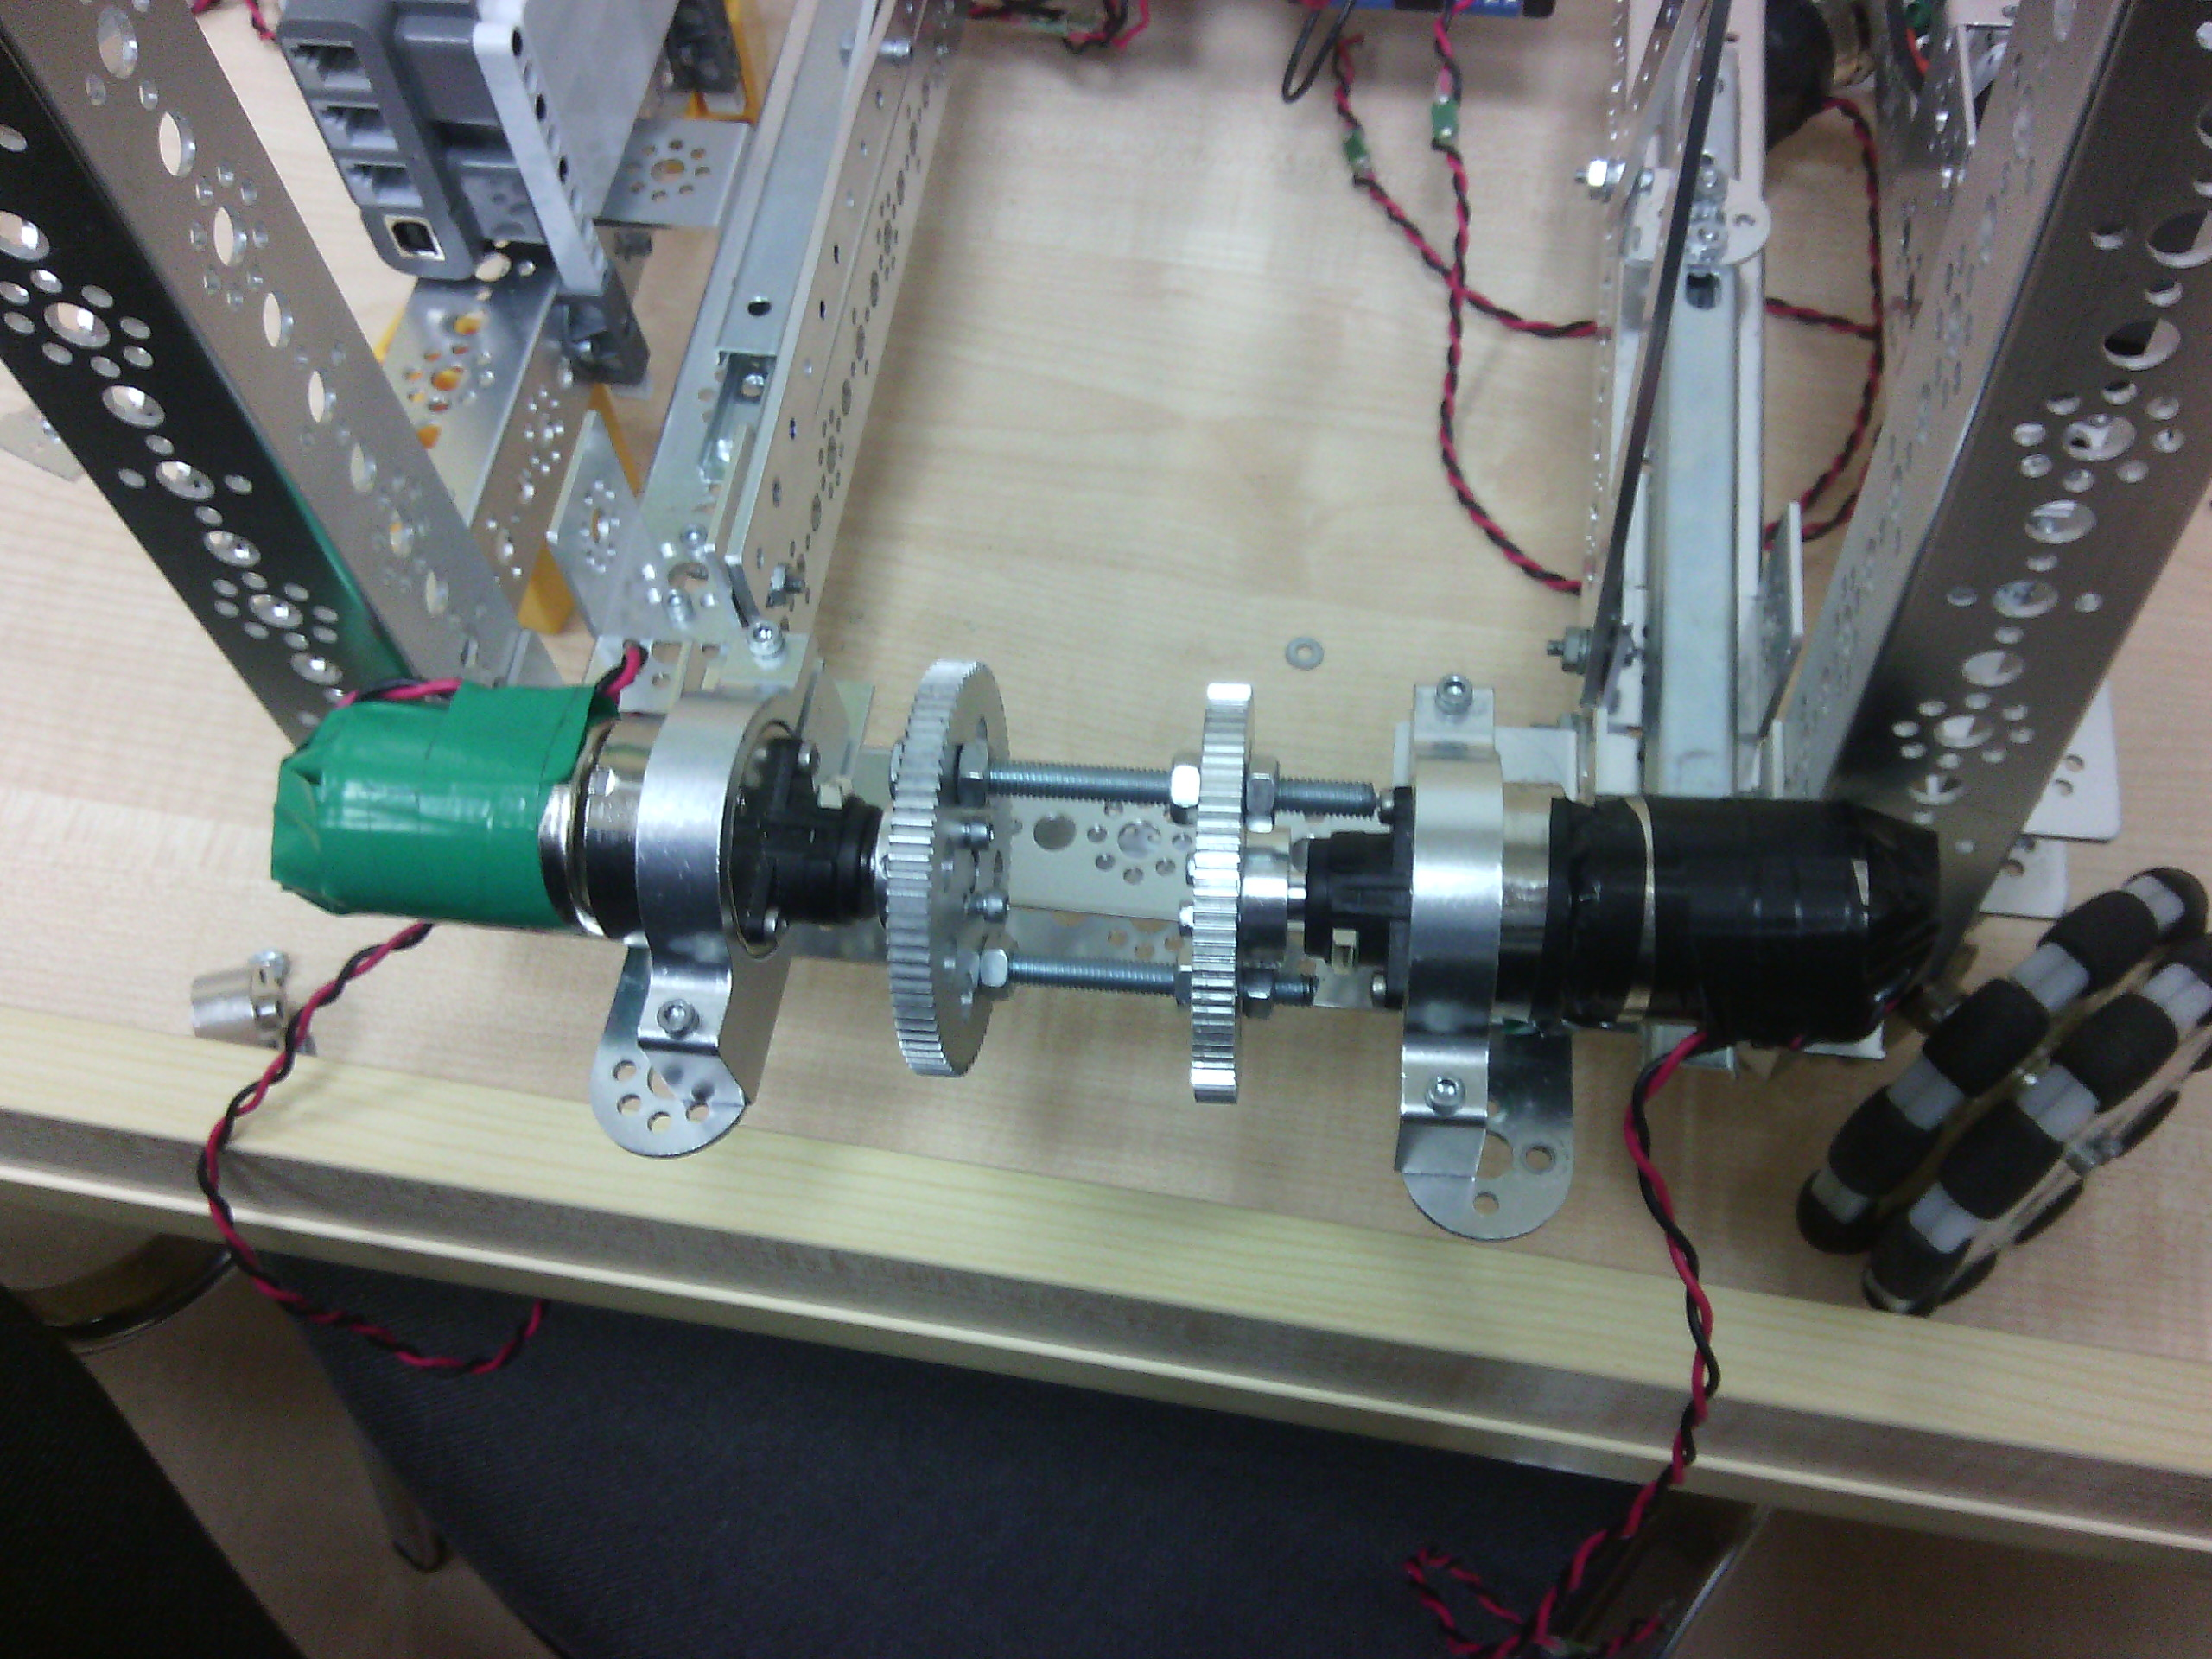
\includegraphics[width=40mm,height=25mm]{Days/13.10.14/5_1_robot}\\ Рисунок 6
			\end{minipage}
			\begin{minipage}{0.3\linewidth}
				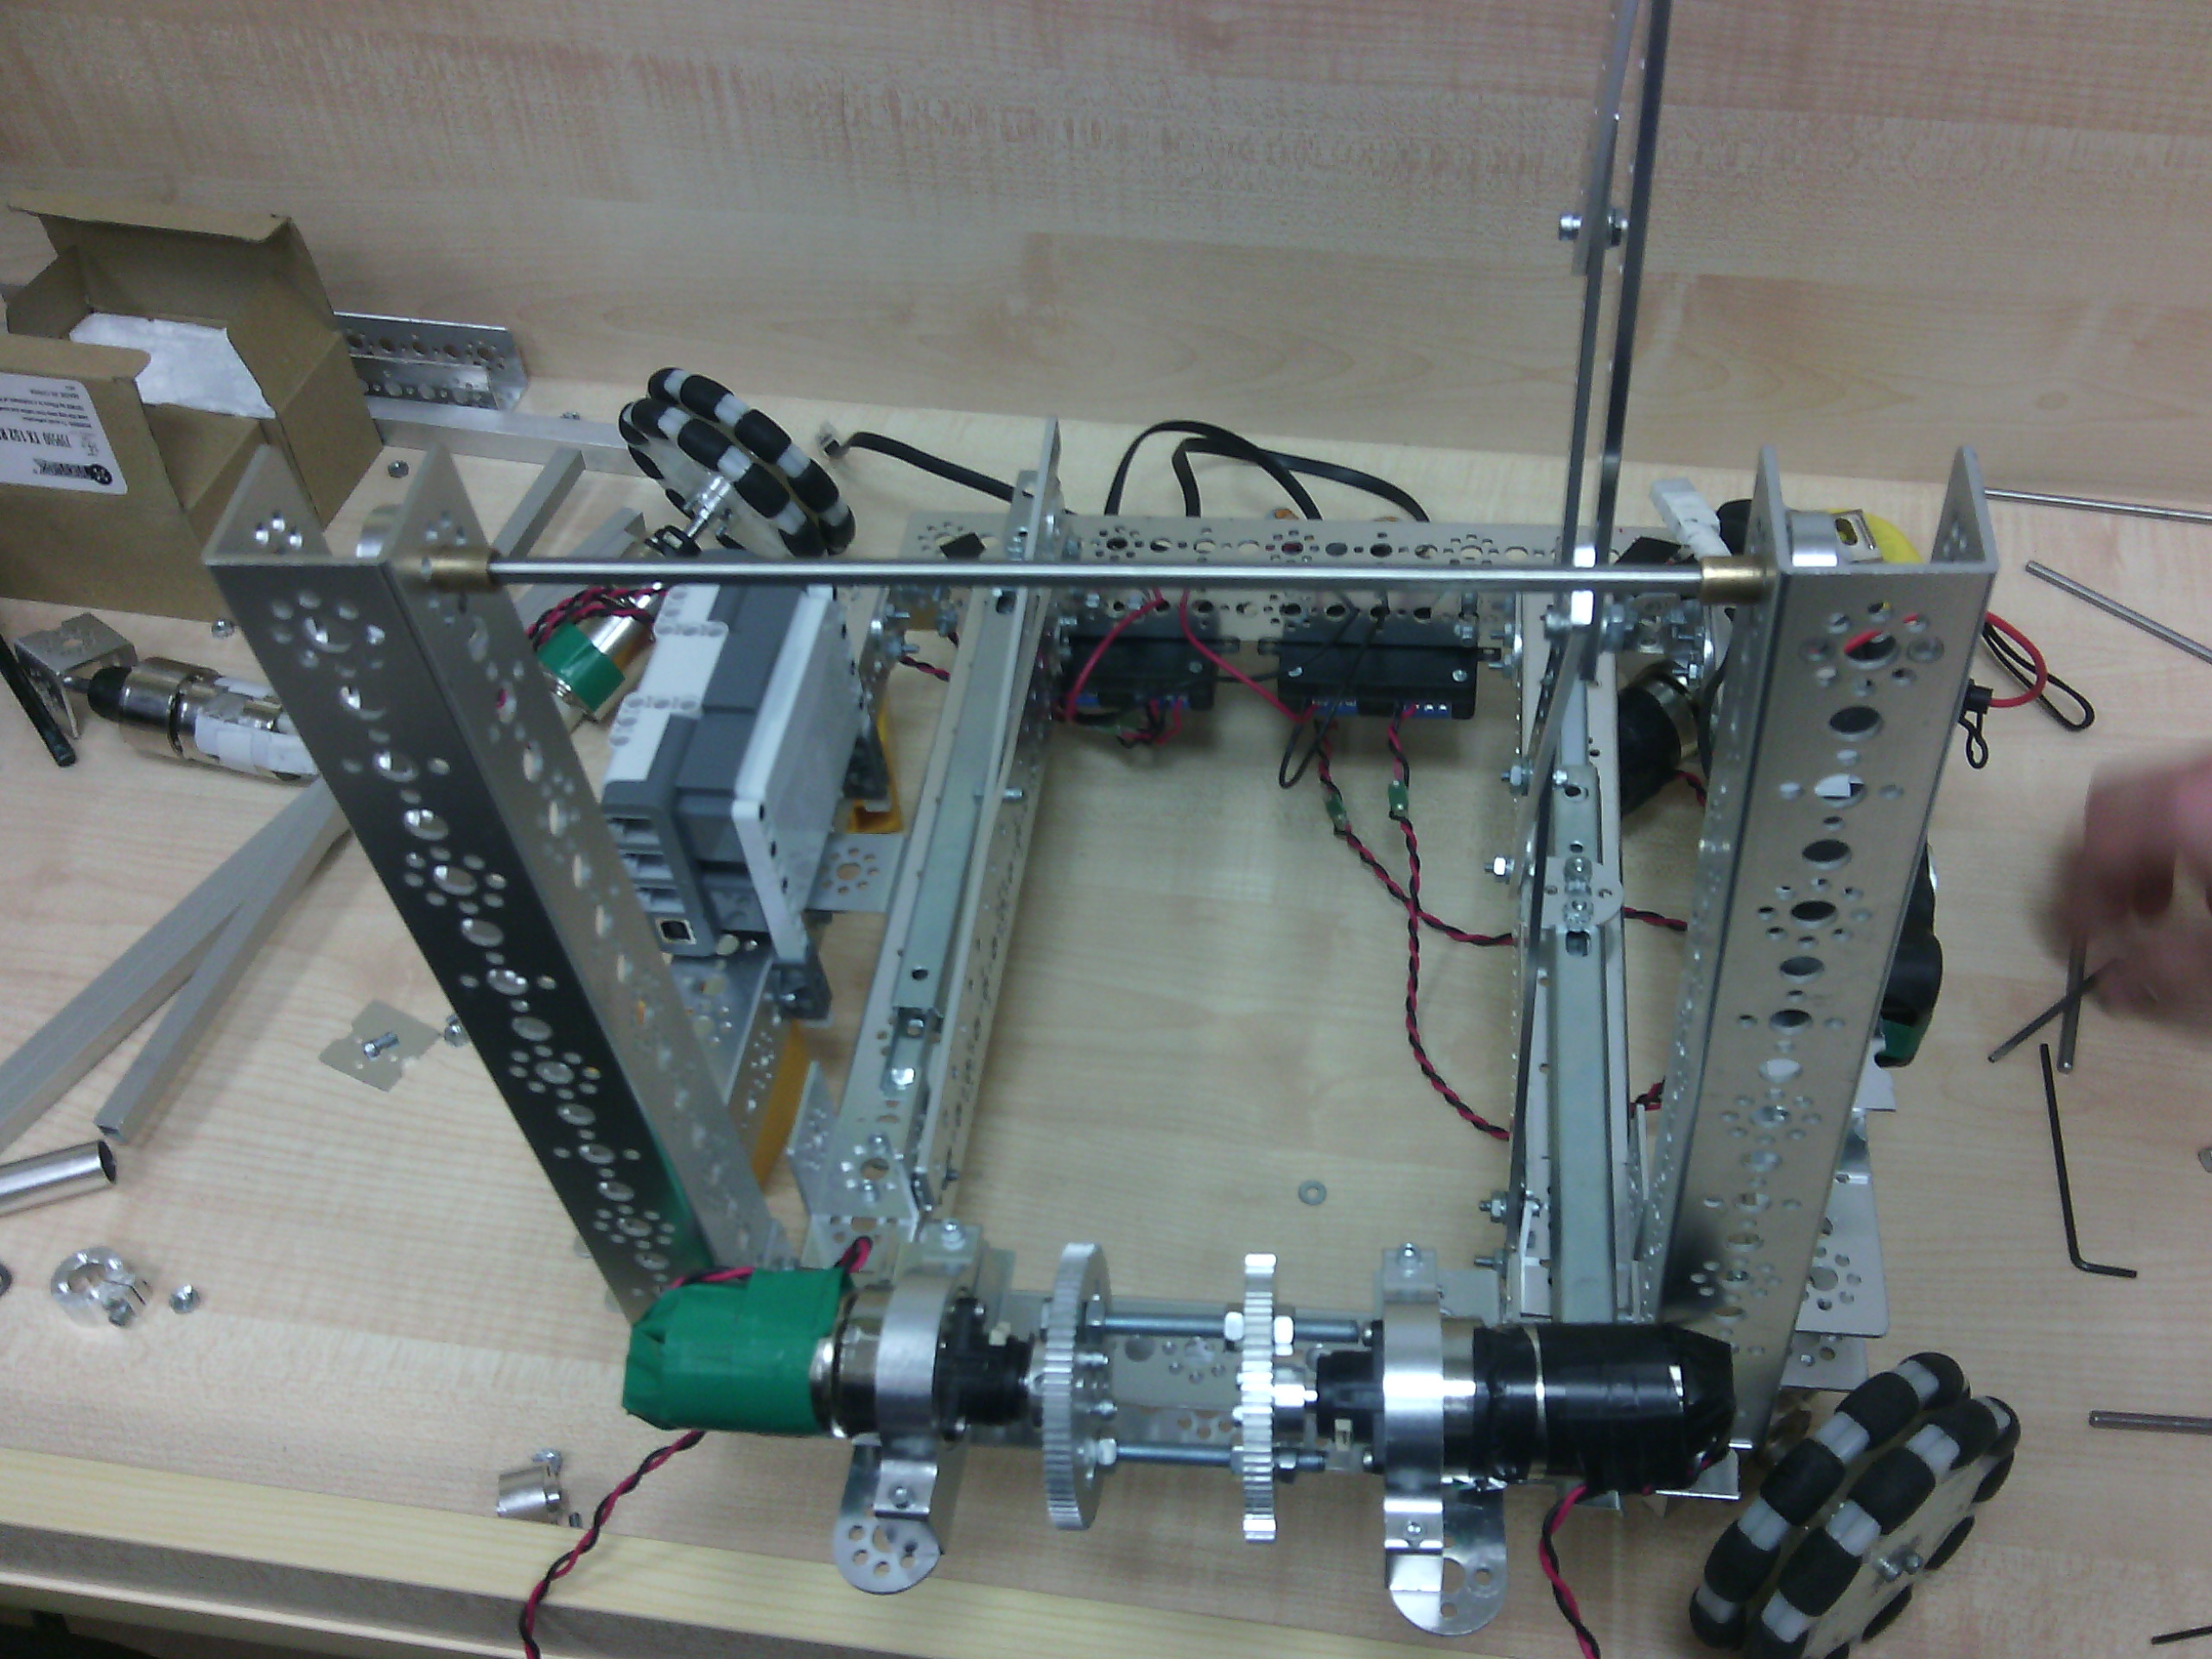
\includegraphics[width=40mm,height=25mm]{Days/13.10.14/5_2_robot}\\ Рисунок 7
			\end{minipage}
		\end{figure}
	\end{enumerate}
	\clearpage
